%%%%%%%%%%%%%%%%%%%%%% CHAPTER ONE %%%%%%%%%%%%%%%%%%%%%%%%%%%%%%%%%%%%%%%
\chapter{Installing Rocks}

\section{Rocks Installation}
We advise you to go through the rocks official \cite{rocksinstall} documentation  before the installation to understand the basic principles of clusters.\\
%Please refer to Appendix I for detailed steps.
\subsection{Physical Assembly}
The first thing to manage is the physical deployment of a cluster.The following diagram shows how the frontend and compute nodes must be connected:

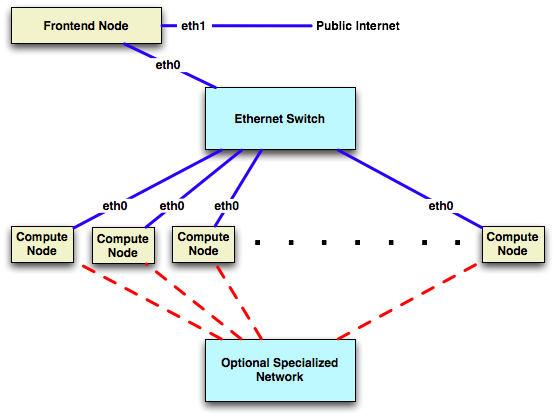
\includegraphics[scale=.5]{cluster.png} 
\paragraph{}
On the Compute nodes (Vm-container), the Ethernet interface that Linux maps to eth0 should be connected to the cluster's Ethernet switch. This network is considered private, i.e, all traffic on this network is physically separated from the external public network (e.g., The Internet).
On the Frontend, at least two Ethernet interfaces are required. The interface that Linux maps to eth0 should be connected to the same Ethernet network as the compute nodes. The interface that Linux maps to eth1 should be connected to the external network (Internet or your organization's intranet).
\paragraph{}
In our case the eth0 is connected to the switch placed within the rack and eth1 of the Frontend is connected to public network under Networks systems lab’s subnet.

\section{Frontend Installation}
The installation on the Frontend is done using a disk image either by a DVD or a bootable USB drive.The Jumbo DVD has all the required rolls in one single disk image. The x86 64 version of Rocks 6.1 can be downloaded from here \cite{rocksdownload}

\begin{itemize}
\item Insert the DVD/USB Drive and restart the main node (Frontend). A boot screen will be displayed with a prompt. Enter the following command to start the installation: 
 \item The next screen shows the list of all rolls in the DVD. Select the required rolls from the list. The Kernel, Base, OS and Web-Server rolls are mandatory. Additional rolls can be installed by using DVD based rolls. Hit next to proceed.
\item The next screen is for entering Cluster Information. Enter the details for Host name, cluster name, organization, locality, state, country, contact, URL, latitude and longitude. The fully-qualified host name is mandatory and is important for several cluster services.
 \item The next screen has the option to set the eth1 ( which is the interface to public network ) IP address. This is the public IP of the cluster(connected to the internet). Enter the public IP as 192.168.41.203.
 
\item The next screen has the option to set the private network eth0 IP address and netmask. This is the IP address of the private network between the Frontend and the nodes. The IP address used is 10.1.1.1 and the netmask is 255.255.0.0.

\item Now configure the gateway and DNS. Gateway used is 192.168.41.1 and DNS servers used are 192.168.254.2, 192.168.254.3.

\item Enter the root password of the cluster when prompted.
\item Configure the time by selecting the time zone for the cluster followed by inputting a Network Time Protocol(NTP) server that will keep the clock on the frontend in sync.

\item The next screen shows the option for the partitioning of the hard disk of the Frontend. Select "Manual Partitioning" since the configuration of " Auto Partitioning provides insufficient space for the /var partition which is used by the Eucalyptus Cloud to upload Virtual Machine Images.

\item The partition used for frontend is: \\ 
\end{itemize}

\begin{center}
\begin{tabular}{ | l | c | r |}
    \hline
    Partition Name & Size  \\ \hline
    /&170GB \\ 
    /var&480GB \\
	/export&170GB \\
	swap&1GB    \\
    \hline
  \end{tabular}
\end{center}
%%%%%%%%%%%%%%%%%%%%%% END OF CHAPTER ONE %%%%%%%%%%%%%%%%%%%%%%%%%%%%%%%%%%%%%%%

%%%%%%%%%%%%%%%%%%%%%CHAPTER 2 INTRO TO EUCA%%%%%%%%%%%%%%%%%%%%%%%%%%%%%%%%%%%%%
\chapter{Introduction to Eucalyptus}

Eucalyptus is a Linux-based software architecture that implements scalable private and hybrid clouds within your existing IT infrastructure. Eucalyptus allows you to provision your own collections of resources (hardware, storage, and network) using a self-service interface on an as-needed basis. \linebreak
\\
You deploy a Eucalyptus cloud across your enterprise’s on-premise data center. Users access Eucalyptus over your enterprise's intranet. This allows sensitive data to remain secure from external intrusion behind the enterprise firewall.
\linebreak

You can install Eucalyptus on the following Linux distributions:
\begin{itemize}
\item CentOS 6
\item Red Hat Enterprise Linux 6
\end{itemize}

\section{Overview}
Eucalyptus was designed to be easy to install and as non-intrusive as possible. The software framework is modular, with industry-standard, language-agnostic communication. Eucalyptus provides a virtual network overlay that both isolates network traffic of different users and allows two or more clusters to appear to belong to the same Local Area Network (LAN). Also, Eucalyptus offers API compatibility with Amazon’s EC2, S3, and IAM services. This offers you the capability of a hybrid cloud.

\section{Eucalyptus Components}
Eucalyptus is comprised of six components: Cloud Controller (CLC), Walrus, Cluster Controller (CC), Storage Controller (SC), Node Controller (NC) and an optional VMware Broker (Broker or VB). Other than the VMware Broker, each component is a stand-alone web service. This architecture allows Eucalyptus both to expose each web service as a well-defined, language-agnostic API, and to support existing web service standards for secure communication between its components.
A detailed description of each Eucalyptus component follows.\linebreak
\subsection{Cloud Controller}
The Cloud Controller (CLC) is the entry-point into the cloud for administrators, developers, project managers, and end-users. The CLC queries other components for information about resources, makes high-level scheduling decisions, and makes requests to the Cluster Controllers (CCs). As the interface to the management platform, the CLC is responsible for exposing and managing the underlying virtualized resources (servers, network, and storage). You can access the CLC through command line tools that are compatible with Amazon’s Elastic Compute Cloud (EC2) and through a web-based Eucalyptus Administrator Console.
\subsection{Walrus}
Walrus allows users to store persistent data, organized as buckets and objects. You can use Walrus to create, delete, and list buckets, or to put, get, and delete objects, or to set access control policies. Walrus is interface compatible with Amazon’s Simple Storage Service (S3), providing a mechanism for storing and accessing virtual machine images and user data. Walrus can be accessed by end-users, whether the user is running a client from outside the cloud or from a virtual machine instance running inside the cloud.
\subsection{Cluster Controller}
The Cluster Controller (CC) generally executes on a machine that has network connectivity to both the machines running the Node Controllers (NCs) and to the machine running the CLC. CCs gather information about a set of NCs and schedules virtual machine (VM) execution on specific NCs. The CC also manages the virtual machine networks. All NCs associated with a single CC must be in the same subnet.
\subsection{Storage Controller}
The Storage Controller (SC) provides functionality similar to the Amazon Elastic Block Store (Amazon EBS). The SC is capable of interfacing with various storage systems. Elastic block storage exports storage volumes that can be attached by a VM and mounted or accessed as a raw block device. EBS volumes persist past VM termination and are commonly used to store persistent data. An EBS volume cannot be shared between VMs and can only be accessed within the same availability zone in which the VM is running. Users can create snapshots from EBS volumes. Snapshots are stored in Walrus and made available across availability zones. Eucalyptus with SAN support lets you use your enterprise-grade SAN devices to host EBS storage within a Eucalyptus cloud.
\subsection{Node Controller}
The Node Controller (NC) executes on any machine that hosts VM instances. The NC controls VM activities, including the execution, inspection, and termination of VM instances. It also fetches and maintains a local cache of instance images, and it queries and controls the system software (host OS and the hypervisor) in response to queries and control requests from the CC. The NC is also responsible for the management of the virtual network endpoint.
\section{Understanding the Eucalyptus Architecture}
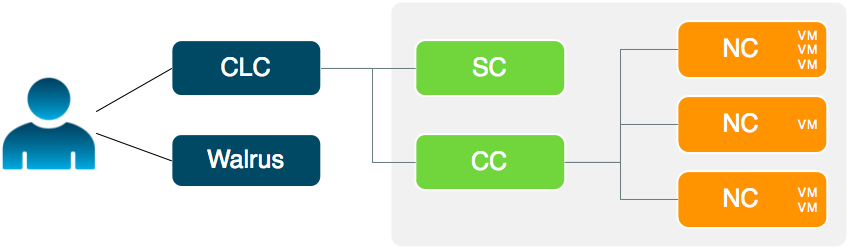
\includegraphics[scale=0.75]{euca-arch.png} 
\linebreak
The cloud components, Cloud Controller (CLC) and Walrus, communicate with cluster components, the Cluster Controllers (CCs) and Storage Controllers (SCs). The CCs and SCs, in turn, communicate with the Node Controllers (NCs). The networks between machines hosting these components must be able to allow TCP connections between them.
\\ \\
However, if the CCs are on separate network interfaces (one for the network on which the cloud components are hosted and another for the network that NCs use) the CCs will act as software routers between these networks in some networking configurations. So each cluster can use an internal private network for its NCs and the CCs will route traffic from that network to a network shared by the cloud components.
\\ \\
Virtual machines (VMs) run on the machines that host NCs. You can use the CCs as software routers for traffic between clients outside Eucalyptus and VMs. Or the VMs can use the routing framework already in place without CC software routers. However, depending on the layer-2 isolation characteristics of your existing network, you might not be able to implement all of the security features supported by Eucalyptus. 
\\ \\
Note : In our cluster we have installed CC, Walrus, CLC, SC in the frontend and the NC’s in the nodes.
%%%%%%%%%%%%%%%%%%%%%%%%%END OF CHAPTER 2%%%%%%%%%%%%%%%%%%%%%%%%%%%%%%%%%%%%%%%%%%%%%%%%%%%%%%%%%%%


